% !TEX TS-program = pdflatex

%%%%%%%%%% NO MODIFICAR  %%%%%%
\documentclass[journal]{IEEEtran}
\IEEEoverridecommandlockouts

%%%%%%%%%%%%%%%%%%%%%%%%%%%%%%%%%%%%%%
%%%%%%%% PRINCIPALES PAQUETES %%%%%%%%
%      No modificar esta area        %
%%%%%%%%%%%%%%%%%%%%%%%%%%%%%%%%%%%%%%
\usepackage{fancyhdr}
\usepackage{graphicx}
\usepackage[utf8]{inputenc}
\usepackage{color}
%\usepackage{hyperref}
\usepackage[hidelinks]{hyperref} 
\usepackage{wrapfig}
\usepackage{array}
\usepackage{multirow}
\usepackage{adjustbox}
\usepackage{nccmath}
\usepackage{subfigure}
\usepackage{amsfonts,latexsym} % para tener disponibilidad de diversos simbolos
\usepackage{enumerate}
\usepackage{booktabs}
\usepackage{float}
\usepackage{threeparttable}
\usepackage{array,colortbl}
\usepackage{ifpdf}
\usepackage{rotating}
%\usepackage{cite}
\usepackage{stfloats}
\usepackage{url}
\usepackage{listings}
%%%%%%%%%%%%%%%%%%%%%%%%%%%%%%%%%%%%%%%%%%%


%%%%%%%%%%%%%%%%%%%%%%%%%%%%%%%%%%%%%%%%%%%
%%% CREAR Y REESCRIBIR ALGUNOS COMANDOS %%%
%              No modificar esta area     %
%%%%%%%%%%%%%%%%%%%%%%%%%%%%%%%%%%%%%%%%%%%
\renewcommand\IEEEkeywordsname{Palabras clave}
%%%%%%%%%%%%%%%%%%%%%%%%%%%%%%%%%%%%%%%%%%%



%%%%%%%%%%%%%%%%%%%%%%%%%%%%%%%%%%%%%%%%%%%
%%%           CONFIGURACION             %%%
%              No modificar esta area     %
%%%%%%%%%%%%%%%%%%%%%%%%%%%%%%%%%%%%%%%%%%%
% correct bad hyphenation here
\hyphenation{op-tical net-works semi-conduc-tor} %% Con este comando se especifican como pueden seprarse las sílabas adecuadamente en caso una palabra quede en dos lineas diferentes de texto

\graphicspath{ {figs/} }  %%Ruta donde se encuentran las imágenes, que esté vacio indica que las imagenes están dentro de la misma carpeta que contiene el archivo .tex
%%%%%%%%%%%%%%%%%%%%%%%%%%%%%%%%%%%%%%%%%%

%%%%%%%%%%%%%%%%%%%%%%%%%%%%%%%%%%%%%%%%%%%%%%%%%%%%%%%%%%
%%% ENCABEZADO DE LAS PÁGINAS TIPO UNIVERSIDAD CENTRAL %%%
%%%%%%%%%%%%%%%%%%%%%%%%%%%%%%%%%%%%%%%%%%%%%%%%%%%%%%%%%%
\newcommand{\MYhead}{\smash{\scriptsize
\hfil\parbox[t][\height][t]{\textwidth}{\centering
\begin{picture}(-100,0) \put(-140,-20){
\includegraphics[width=40mm]{logoing}} \end{picture} \hspace{6.4cm}
COLORADO SCHOOL OF MINES\\ 
\hspace{2.8cm} GEOPHYSICS DEPARTMENT, RESERVOIR CHARACTERIZATION PROJECT
% REPORTE DE PRÁCTICA DE LABORATORIO \hspace{5.15cm} Versión 1\\
% \hspace{2.8cm} LABORATORIO DE ELECTRÓNICA. ÁREA MECÁNICA ELÉCTRICA, FACULTAD DE INGENIERÍA - UASLP \hspace{1cm} Periodo 2022-2023I\\
}\hfil\hbox{}}}
\makeatletter
% normal pages
\def\ps@headings{%
\def\@oddhead{\MYhead}%
\def\@evenhead{\MYhead}}%
% title page
\def\ps@IEEEtitlepagestyle{%
\def\@oddhead{\MYhead}%
\def\@evenhead{\MYhead}}%
\makeatother
% make changes take effect
\pagestyle{headings}
% adjust as needed
\addtolength{\footskip}{0\baselineskip}
\addtolength{\textheight}{-1\baselineskip}
%%%%%%%%%%%%%%%%%%%%%%%%%%%%%%%%


%%%%% INICIO DEL DOCUMENTO %%%%%
%      AREA CONFIGURABLE       %
%%%%%%%%%%%%%%%%%%%%%%%%%%%%%%%%
\begin{document}

%Titulo
\title{\textcolor{black}{Report on 10.2-10.8}}      

%Datos
\author{Shenyao Jin} 


\maketitle


\section{Code Snapshot}
\begin{verbatim}
# Homework 1, CV
# Shenyao Jin, shenyaojin@mines.edu
#%% Import libs
import numpy as np
import matplotlib.pyplot as plt
from skimage.io import imread
#%% Define data path
data_path = "./data/IMG_5167.jpeg"

#%% Load image
image = imread(data_path)
rotated_image = np.rot90(image, k=3) # Need to rotate the image
#%% Show image
plt.figure()
plt.imshow(rotated_image)
plt.axis("off")
plt.show()

#%% Change the dtype to float32 and convert into grayscale
image_float = rotated_image.astype(np.float32)
image_gray = np.dot(image_float, [0.299, 0.587, 0.114])

#%% Show grayscale image
plt.figure()
plt.imshow(image_gray, cmap='gray')
plt.axis("off")
plt.show()

#%% Print the top left (3*5) pixels of the grayscale image
print(image_gray[:3,:5])

#%% Print index=(1,2) of image_gray. We assume the index start from 1.
print(image_gray[0,1])
\end{verbatim}

\section{Grayscale Image Snapshot}
\begin{figure}[h]
    \centering
    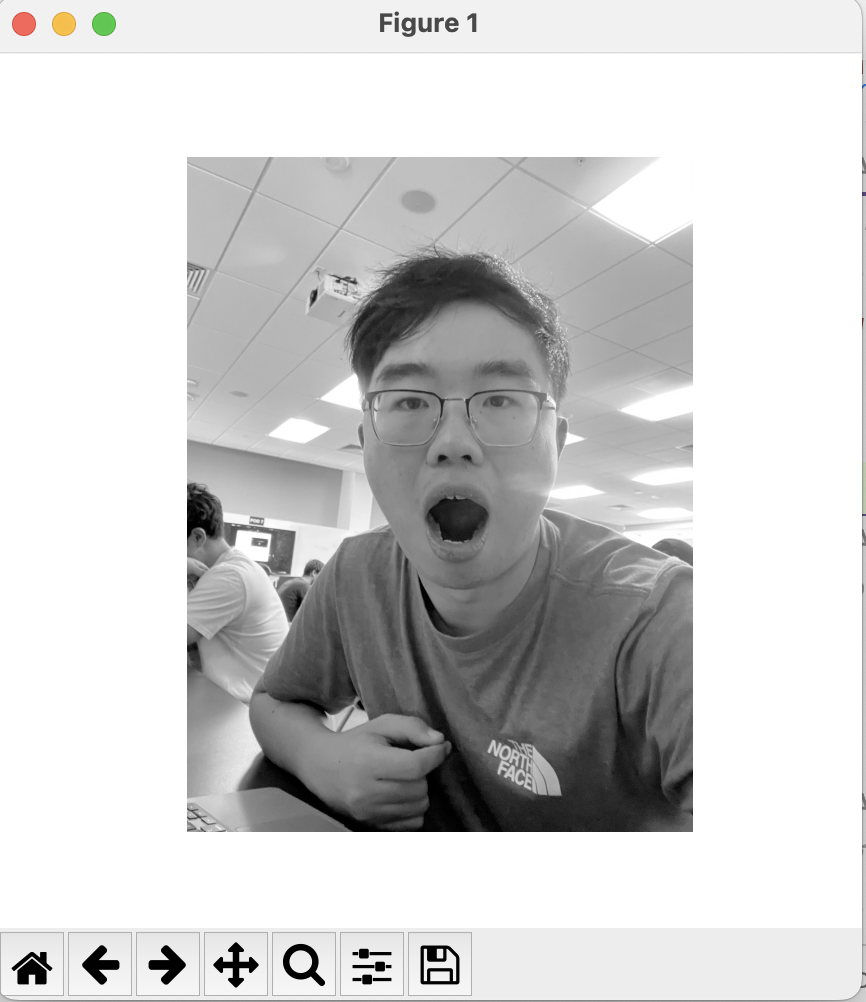
\includegraphics[width=0.8\columnwidth]{../data/gray_scale_figure.png}
    \caption{Grayscale Image}
\end{figure}

\section{Pixel Values}

\subsection{Top Left 3x5 Matrix}
\begin{verbatim}
[[179.789 180.789 177.789 172.789 170.789]
 [178.789 178.789 176.789 174.789 171.789]
 [179.789 178.789 177.789 177.789 177.789]]
\end{verbatim}

\subsection{Pixel at (1,2)}
The value of the pixel at index (1,2) is 180.789.


%%%%%%%%%%%%%%%%%%%%%%%%%%%%%%%
%%%%%%%%%%%%%%%%%%%%%%%%%%%%%%%
\end{document}






